\section{Git}

\section{Getting started}

\begin{frame}
  \frametitle{A couple of Quotes}
  {\scriptsize
  \begin{quote}
    ``For the first 10 years of kernel maintenance, we literally used
    tarballs and patches, which is a much superior source code
    management system than CVS is[...]'' -- Linus Torvalds
  \end{quote}

  \begin{quote}
    ``When I say I hate CVS with a passion, I have to also say that if
    there any SVN users in the audience, you might
    want to leave. Because my hatred of CVS has meant that I see
    Subversion as being the most pointless project ever started,
    because the whole slogan for the Subversion for a while was 'CVS
    done right' or something like that. And if you start with that
    kind of slogan, there is nowhere you can go. It's like, there is
    no way to do CVS right.'' -- Linus Torvalds
  \end{quote}
}
\end{frame}

\begin{frame}[fragile]
  \frametitle{First of all}
  \begin{itemize}
  \item Telling git who you are
    {\scriptsize
\begin{verbatim}
[user]
        name = Your Name
        email = your@mail.ext
\end{verbatim} 
    }
    \begin{itemize}
    \item Global: \verb|~/.gitconfig|
    \item Repository specific: \verb|repodir/.git/config|
    \end{itemize}
  \item Extensible config file
  \item git-config command
  \end{itemize}
\end{frame}

\begin{frame}[fragile]
  \frametitle{Basic operations}
  \begin{itemize}
  \item Creating/Initializing a new repository
    {\scriptsize
\begin{verbatim}
$ mkdir project
$ cd project
$ git init
\end{verbatim}
    }

  \item Committing
    {\scriptsize
\begin{verbatim}
$ git add file
$ git commit 
\end{verbatim}
    }

  \item Differences
    \begin{itemize}
    \item {\scriptsize \verb|git diff|}: differences between the work tree and the index
    \item {\scriptsize \verb|git diff --cached|}: differences between HEAD and the index
    \end{itemize}

  \item Special shortcut for committing
    {\scriptsize
\begin{verbatim}
$ git commit -a
\end{verbatim}
    }

  \item Status
    {\scriptsize
\begin{verbatim}
$ git status
\end{verbatim}
    }
  \end{itemize}

NOTE: the index is a snapshot of the working tree that represents the
content that will be affected by a commit
\end{frame}

\begin{frame}[fragile]
  \frametitle{Fixing mistakes}

  \begin{itemize}
  \item Resetting by changing the history
    {\scriptsize
\begin{verbatim}
$ git reset --hard <commit>
\end{verbatim}
      }

    \item Reverting with a new commit
      {\scriptsize
\begin{verbatim}
$ git revert <commit>
\end{verbatim}
      }

    \item Getting an old version of a file
      {\scriptsize
\begin{verbatim}
$ git checkout <commit> path/to/file
\end{verbatim}
      }
      \end{itemize}

\end{frame}

\section{Exploring the history}

\begin{frame}[fragile]
  \frametitle{Exploring the history}

  \begin{itemize}
  \item {\it git log}
    {\scriptsize
\begin{verbatim}
commit ce6ddeac2200225b173c52e2509ffcc01b2b4a1d
Author: Carlos Garcia Campos <carlosgc@gnome.org>
Date:   Mon Nov 19 16:14:01 2007 +0100

    Initial commit
\end{verbatim}
    }


    \begin{itemize}
    \item Commit: commit id (sha1)
    \item Author: commit author (not the committer)
    \item Date: commit date
    \item Commit message: (a single line briefly 
      describing the change and, optionally, a blank line followed by
      one or more lines with a detailed description)
    \end{itemize}
  \end{itemize}

  ChangeLog file is no longer needed. 

\end{frame}

\begin{frame}[fragile]
  \frametitle{Customizing the log command output}

  \begin{itemize}

  \item Change stats: {\scriptsize{\it \verb|--stat|}}
  \item Diff of the changes (patch): {\scriptsize{\it \verb|-p|}}
  \item With information about the altered paths: {\scriptsize{\it \verb|--name-status|}}
  \item Wit full information about both the Author and Committer: {\scriptsize{\it \verb|--pretty=fuller|}}
  \item Limiting the amount of commits shown : {\scriptsize{\it \verb|-n<n_commits>|}}
  \item Useful shortcut: {\scriptsize{\it \verb|git show|}}
  \end{itemize}

\end{frame}

\begin{frame}
  \frametitle{Git internals}

  \begin{itemize}
  \item The whole history of the repository is stored by Git in files
    referenced by its contents (SHA1) rather than a file name. 
  \item Such files are the ``objects'' that form the Git Object Model.
  \item Every object consists of a type, a size and its contents.
  \item Four types of objects:
    \begin{itemize}
    \item {\bf blob} is just a file
    \item {\bf tree} is a container of pointers to blobs and other
      tree objects
    \item {\bf commit} is a link to a physical state of a tree with a
      description of how we got there and why
    \item {\bf tag} is used to mark commit objects with a label
    \end{itemize}
  \end{itemize}
\end{frame}

\begin{frame}
  \frametitle{The Git Object Model (Example)}
  \begin{center}
    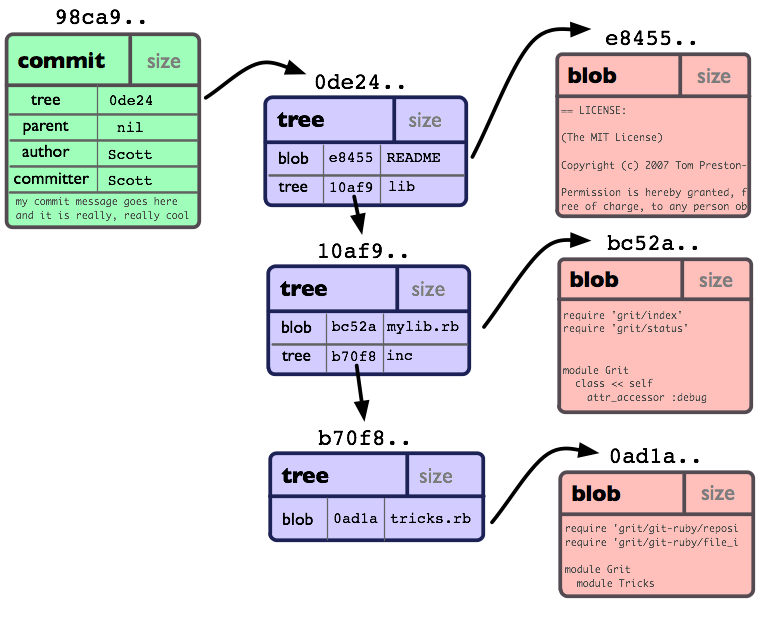
\includegraphics[width=7cm]{figs/objects-example.png}
  \end{center}

{\Tiny
Image from Git Community Book
(\url{http://book.git-scm.com/index.html})
}
\end{frame}

\section{Branching and Merging}

\begin{frame}[fragile]
  \frametitle{Working with branches}

  \begin{itemize}
  \item Branches are quite ``cheap'' (fast and clean process)
  \item Creating a new branch
    {\scriptsize
\begin{verbatim}
$ git branch <branch> [<start-point>]
\end{verbatim}
    }

  \item Listing available branches
    {\scriptsize
\begin{verbatim}
$ git branch
\end{verbatim}
    }

  \item Changing the current branch
    {\scriptsize
\begin{verbatim}
$ git checkout
\end{verbatim}
    }

  \item Creating a branch and changing to it in a single operation
    {\scriptsize
\begin{verbatim}
$ git checkout -b <branch> [<start-point>]
\end{verbatim}
    }      

  \item Merging branches
    {\scriptsize
\begin{verbatim}
$ git merge <branch>
\end{verbatim} 
    }

  \item Updating the current branch from another
    {\scriptsize
\begin{verbatim}
$ git rebase <branch>
\end{verbatim}
    }
  \end{itemize}
\end{frame}

\section{Operations between repositories}

\begin{frame}[fragile]
  \frametitle{Pulling}

  \begin{itemize}
  \item Cloning a repository (clone != checkout)
    {\scriptsize
\begin{verbatim}
$ git clone <uri>
\end{verbatim}
    }

  \item Getting updates
    {\scriptsize
\begin{verbatim}
$ git fetch <uri>
$ git merge origin/master
\end{verbatim}
    }

  \item Useful shortcut (commonly used)
    {\scriptsize
\begin{verbatim}
$ git pull
\end{verbatim}
    }

  \item Updating a remote repository
    {\scriptsize
\begin{verbatim}
$ git push
\end{verbatim}
    }

  \end{itemize}
\end{frame}

\begin{frame}[fragile]
  \frametitle{Workflow (Summary)}
  {\scriptsize
\begin{verbatim}
$ git clone <uri>
$ cd project
$ git checkout -b new-feature
(some changes, git add, etc.)
$ git commit -a
(more changes)
$ git commit -a
(last changes, my new feature is now ready)
$ git commit -a
$ git checkout master
$ git pull
$ git checkout new-feature
$ git rebase master
$ git checkout master
$ git merge new-feature
$ git push origin master
\end{verbatim}
  }
\end{frame}

\begin{frame}
  \frametitle{Big advantages for the daily work}

  \begin{itemize}
  \item Offline work
    \pause
  \item Working on more than one feature at the same time
    \pause
  \item Micro-commits
    \pause
  \item Easy sharing of code
    \pause
  \item Author != Committer
    \pause
  \item Better history
    \pause
  \item Interactivity with other systems (git-svn, git-cvs)
    \pause
  \item {\bf Performance!!!}
  \end{itemize}
\end{frame}

\begin{frame}[fragile]
  \frametitle{Patches}

  \begin{itemize}
  \item Creating series of patches
    {\scriptsize
\begin{verbatim}
$ git format-patch <commit-from>..<commit-to>
\end{verbatim}
    }

  \item Appliying series of patches
    {\scriptsize
\begin{verbatim}
$ cat patch1 patch2 .. patchn > patches.mbox
$ git am patches.mbox
\end{verbatim}
    }
    \end{itemize}

\end{frame}


